\section{The Domain Shift Challenge}
\label{sec:3.4}

The machine learning classification methods introduced in Section~\ref{sec:3.3} are built on the implicit assumption that the training data faithfully represent the conditions under which the model will be deployed.
When this assumption breaks down---as it does for several astrophysical classification tasks---the standard approaches described in the previous sections require modification.
We now turn to the problem of \textit{dataset shift}, a systematic mismatch between training and target distributions that, if left unaddressed, can bias inference results.
We first formalize the problem (Section~\ref{sec:3.4.1}) and then describe its principal types and the strategies used to correct them (Section~\ref{sec:3.4.2}).

\subsection{The Problem Statement}
\label{sec:3.4.1}

Supervised classification algorithms rely on the assumption that the training data and the target data share the same joint probability distribution of input features $\mathbf{x}$ and output classes $k$:
\begin{equation}
	p_{\text{train}}(\mathbf{x}, k) = p_{\text{target}}(\mathbf{x}, k).
	\label{eq:dataset_shift_assumption}
\end{equation}
When this condition holds, a classifier trained on labeled examples can be applied directly to unlabeled data with the expectation that its performance will generalize.
In practice, however, this assumption is frequently violated.
A mismatch between the training and target distributions---known as \textit{dataset shift} \cite{MorenoTorres2012AUV}---invalidates the direct application of the trained model and can produce systematically biased estimates of class prevalences and, consequently, incorrect statistical constraints on physical parameters.

This problem is directly relevant for astrophysical source classification.
In the Fermi-LAT catalogs, sources are divided into \textit{associated} and \textit{unassociated} categories based on whether a counterpart at other wavelengths has been identified.
Machine learning classifiers are typically trained on associated sources---whose class labels (e.g., pulsar or active galactic nucleus) are known from their multi-wavelength counterparts---and then applied to unassociated sources to infer their nature.
However, several observational biases break the equal-distribution assumption.
Bright sources at high Galactic latitudes are easier to associate with known counterparts, so the associated sample is not a representative subsample of the full source population \cite{2023RASTI...2..735M}.
As a consequence, the spectral parameter distributions---flux, spectral index $\alpha$, and spectral curvature $\beta$---differ measurably between associated and unassociated sources, as illustrated in Figure~\ref{fig:assoc_unas_distributions} (see Chapter~\ref{ch:5} for the full analysis).
Whether this discrepancy arises from observational selection effects, from genuinely different class compositions, or from a combination of both, cannot be determined a priori; we formalize the relevant types of dataset shift in Section~\ref{sec:3.4.2}.
Any analysis that ignores this mismatch risks producing biased class prevalence estimates and, in the context of dark matter searches, unreliable upper bounds on the annihilation cross-section.

\begin{figure}[t]
	\centering
	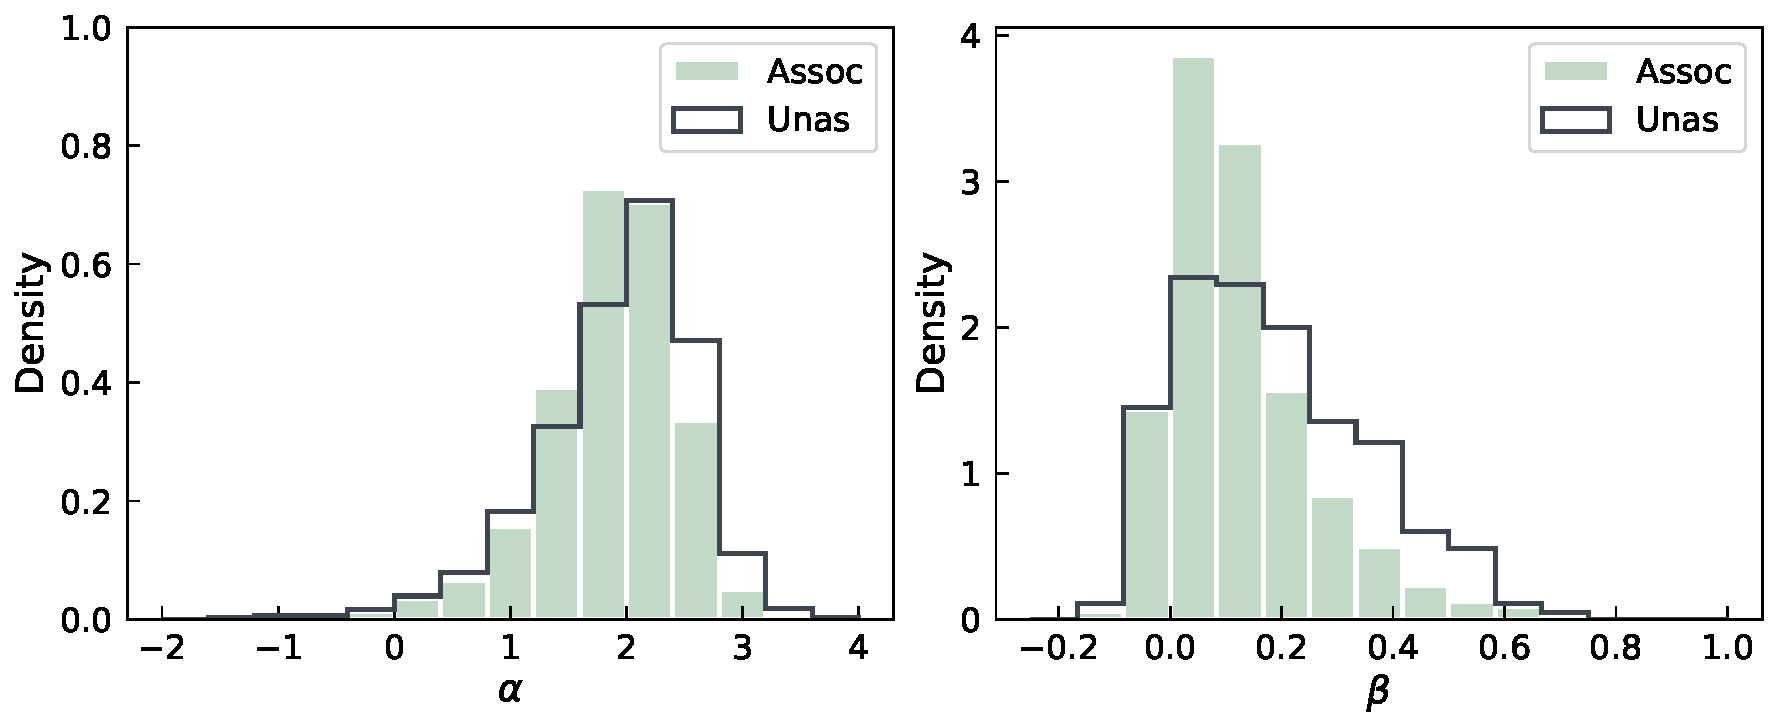
\includegraphics[width=\columnwidth]{chapter_03/figures/alpha_beta_hist_full_range_E01000MeV.pdf}
	\caption{Distributions of the spectral index $\alpha$ and spectral curvature $\beta$ for associated (green, filled) and unassociated (gray outline) Fermi-LAT sources from the 4FGL-DR4 catalog.
		The visible mismatch between the two populations illustrates the dataset shift between the associated and unassociated samples discussed in Section~\ref{sec:3.4.1}.
		The full analysis is presented in Chapter~\ref{ch:5}.
	}
	\label{fig:assoc_unas_distributions}
\end{figure}

\subsection{Types of Dataset Shift}
\label{sec:3.4.2}

The joint distribution of features and class labels can be decomposed in two equivalent ways:
\begin{equation}
	p(\mathbf{x}, k) = p(k|\mathbf{x})\,p(\mathbf{x}) = p(\mathbf{x}|k)\,p(k).
	\label{eq:joint_factorizations}
\end{equation}
These two factorizations give rise to two distinct types of dataset shift, depending on which factor changes between the training and target domains \cite{MorenoTorres2012AUV}.
Each type has distinct statistical consequences and correction strategies.

\paragraph{Covariate shift.}

Covariate shift is most naturally understood through the first factorization, $p(\mathbf{x}, k) = p(k|\mathbf{x})\,p(\mathbf{x})$.
Under this type of shift, the posterior class probabilities given the features remain unchanged between the training and target distributions:
\begin{equation}
	p_{\text{train}}(k|\mathbf{x}) = p_{\text{target}}(k|\mathbf{x}),
	\label{eq:covariate_shift}
\end{equation}
while the marginal distribution of the features differs: $p_{\text{train}}(\mathbf{x}) \neq p_{\text{target}}(\mathbf{x})$ \cite{MorenoTorres2012AUV}.
The class-conditional relationship between features and labels is preserved, but the relative abundance of feature values changes.
Covariate shift typically arises from selection effects or observational biases that influence which data points enter the training sample.
In the Fermi-LAT context, the association procedure preferentially identifies sources in low-background regions far from the Galactic plane, where multi-wavelength counterparts are easier to match.
Proximity to the Galactic plane is, in fact, the dominant source of association bias: the high density of overlapping sources and diffuse emission near the plane causes multi-wavelength identification methods to fail more frequently \cite{2023RASTI...2..735M}.
As a result, the associated sample is biased toward high-latitude, brighter sources relative to the full population.
The ratio $C(\mathbf{x}) = p_{\text{target}}(\mathbf{x})/p_{\text{train}}(\mathbf{x})$ between the target and training feature distributions characterizes the covariate shift \cite{MorenoTorres2012AUV}.
When this ratio is known or can be modeled, the training-set predictions can be corrected by importance weighting.

In practice, $C(\mathbf{x})$ is rarely known analytically, but it can be approximated parametrically.
If the ratio is monotonic in each feature dimension, a product of sigmoid functions provides a physically constrained model that can still accommodate a range of shift shapes:
\begin{equation}
	\tilde{C}(\mathbf{x};\boldsymbol{\theta}_{\text{cov}}) = \prod_{d=1}^{D} f(x_d; b_d, c_d), \qquad f(x_d; b_d, c_d) = \frac{1}{1 + e^{-b_d(x_d - c_d)}},
	\label{eq:sigmoid_modulation}
\end{equation}
where $b_d$ controls the steepness and $c_d$ the midpoint of the modulation along feature dimension $d$ (see Chapter~\ref{ch:5} for the derivation and application).
These parameters are optimized jointly with the rest of the model by maximizing the likelihood of the target data.

\paragraph{Prior shift.}

The prior shift is most clearly seen in the second factorization, $p(\mathbf{x}, k) = p(\mathbf{x}|k)\,p(k)$.
Here, the class-conditional feature distributions are invariant:
\begin{equation}
	p_{\text{train}}(\mathbf{x}|k) = p_{\text{target}}(\mathbf{x}|k),
	\label{eq:prior_shift}
\end{equation}
but the class prevalences differ: $p_{\text{train}}(k) \neq p_{\text{target}}(k)$ \cite{MorenoTorres2012AUV}.
This type of shift is common when the population composition changes between the training and deployment environments.
Among Fermi-LAT sources, for instance, the fraction of Galactic sources is considerably larger in the unassociated sample than in the associated one, because a higher proportion of unassociated sources lie near the Galactic plane \cite{2023RASTI...2..735M}.
Standard classifiers trained with balanced or representative class fractions from the associated data will therefore assign incorrect class probabilities when applied to the unassociated population.
The quantification learning literature \cite{10.1145/3117807_Gonzalez_quantification} addresses this problem by fitting the mixture weights $\pi_k$ of a generative model directly to the target data, rather than relying on the class fractions of the training set \cite{10.1162/089976602753284446_Saerens,2024arXiv240100490M}.

\paragraph{Combined shift.}

In general, covariate and prior shifts act simultaneously, and separating their effects is difficult.
Changes in the marginal class prevalences $p(k)$ produce corresponding changes in the marginal feature distribution $p(\mathbf{x})$, and vice versa, so that the same observed mismatch between training and target distributions can be explained by either mechanism or by both acting together \cite{MorenoTorres2012AUV}.
Resolving this degeneracy requires additional physical constraints or a model flexible enough to fit both effects at once.
A purely covariate-shift correction, for example, might absorb prevalence changes into the reweighting function, while a purely prior-shift model would attribute selection biases to changes in class fractions.
Neither gives the correct answer when both effects are present.

\paragraph{Application preview.}

Addressing this challenge requires a model that treats both effects simultaneously.
In Chapter~\ref{ch:5}, we construct the first such statistical model for Fermi-LAT sources.
The unassociated source distribution is modeled as a mixture of Galactic and extragalactic astrophysical components---whose class-conditional densities $p_{\text{assoc}}(\mathbf{x}|k)$ are estimated from the associated sources via kernel density estimation---plus a possible dark matter subhalo component derived from Monte Carlo simulations.
The prior shift is handled by fitting the class prevalences $\pi_k$ to the unassociated data, while the covariate shift is corrected by the sigmoid modulation functions $\tilde{C}(\mathbf{x};\boldsymbol{\theta}_{\text{cov}})$ described above.
All parameters are optimized simultaneously using the Expectation-Maximization algorithm (Section~\ref{sec:3.3.3}).
This approach draws on the classical dataset shift taxonomy of Moreno-Torres et al.~\cite{MorenoTorres2012AUV} and the quantification learning methods developed by Gonz\'alez et al.~\cite{10.1145/3117807_Gonzalez_quantification} and Moreo et al.~\cite{2024arXiv240100490M}, combining them into a unified framework that can be used both for the probabilistic classification of unassociated sources---its primary astrophysical application---and for setting statistically rigorous upper bounds on the dark matter annihilation cross-section.
The full analysis is presented in Chapter~\ref{ch:5}.
